\documentclass[xcolor=dvipsnames]{beamer}
\useoutertheme{infolines}
\setbeamertemplate{navigation symbols}{}
\setbeamertemplate{items}[ball]
\usepackage{graphicx,multirow,color,xcolor,verbatim,float,comment,amsmath}
\setbeamertemplate{frametitle}[default][center]
\begin{document}
\title{Community Detection in Gene Network}
\author{Bowen Deng}
\institute{Dept. of Prob. and Stat.}
\date{}
\begin{frame}
\maketitle
\end{frame}
\begin{frame}
\tableofcontents
\end{frame}
\section{Optimization Problem}
\begin{frame}{Introduction}
For directed graph, source community and terminal community could be detected with
\[
(\hat{u},\hat{v})=\arg\max u^TQv-\eta(\|u\|_0+\omega\|v\|_0), s.t. \|u\|_2=1, \|v\|_2=1
\]
Source community $SC=\{i|\hat{u}[i]\neq0\}$,\\
Terminal community $TC=\{j|\hat{v}[j]\neq0\}$.\\
\end{frame}
\begin{frame}{Optimization Strategy}
For a given vector $z$ and a fixed constant $\rho>0$, the solution of
\[
\max u^Tz-\rho\|u\|_0, s.t. \|u\|_2=1
\]
is
\[
u=z_l^h/\|z_l^h\|_2
\]
\end{frame}
\begin{frame}
Repeat
\begin{eqnarray}
z\leftarrow Qv, \rho\leftarrow\eta\nonumber\\
u\leftarrow z_l^h/\|z_l^h\|_2,\nonumber\\
z\leftarrow Q^Tu, \rho\leftarrow\eta\omega\nonumber\\
v\leftarrow z_l^h/\|z_l^h\|_2\nonumber
\end{eqnarray}
\end{frame}
\begin{frame}{Undirected Counterpart}
For undirected graph, e.g. gene network, a community could be detected with the symmetric counterpart:\\
\[
\min f(u)=-u^TQu+\rho\|u\|_0, s.t. u^Tu=1
\]
where $Q$ be a fixed symmetric matrix, $\rho$ be a positive number.\\
\end{frame}
\begin{frame}{Mimic Algorithm}
Borrowing the idea from the previous optimization solving,
\begin{eqnarray}
z\leftarrow Qu \nonumber\\
u\leftarrow z_l^h/\|z_l^h\|_2\nonumber
\end{eqnarray}
\end{frame}
\begin{frame}{Brute Force Algorithm}
Fixing $\|u\|_0=k$, the objective is to find a submatrix $|\hat{Q}|=k$ with the largest eigenvalue.\\
For the sake of computational cost, we could also sample the subset with Genetic Algorithm. Once sampled, we find the eigenvalue of the matrix.\\
\end{frame}
\begin{frame}{Variation of the Problem}
\[
\min u^TMu+\rho\|u\|_1, s.t. u^Tu=1
\]
\end{frame}
\begin{frame}{Lagrangian Method}
Consider
\[
\min f(u,l)=u^TMu+\rho\|u\|_1+l(u^Tu-1)
\]
Repeat
\begin{eqnarray}
u\leftarrow u-\lambda\nabla_uf(u,l)\nonumber\\
l\leftarrow l-\lambda\nabla_lf(u,l)\nonumber
\end{eqnarray}
\end{frame}
\section{Relaxation of MWSP}
\begin{frame}{Relaxation}
The original simultaneously detection is
\begin{displaymath}
\begin{split}
\max O(M_1,\cdots,M_t)=\sum_{\rho=1}^t\sum_{i=1}^m(2C_i(M_{\rho})&-\sum_{j=1}^nI_{M_{\rho}}(j)A_{ij})\\
s.t. \sum_{j=1}^nI_{M_{\rho}}(j)A_{ij}&\geqslant C_i(M_{\rho})\\
\sum_{\rho=1}^tI_{M_{\rho}}(j)&\leqslant 1\\
\end{split}
\end{displaymath}
where all variables are binary.\\
The relaxation counterpart is to relax $x\in\{0,1\}$ to $0\leqslant x\leqslant1$.
\end{frame}
\begin{frame}
Set 50 patients, 50 genes, genes 1-4; genes 5-8 are driver pathway genes. Background mutation rate 0.02.\\
\begin{figure}
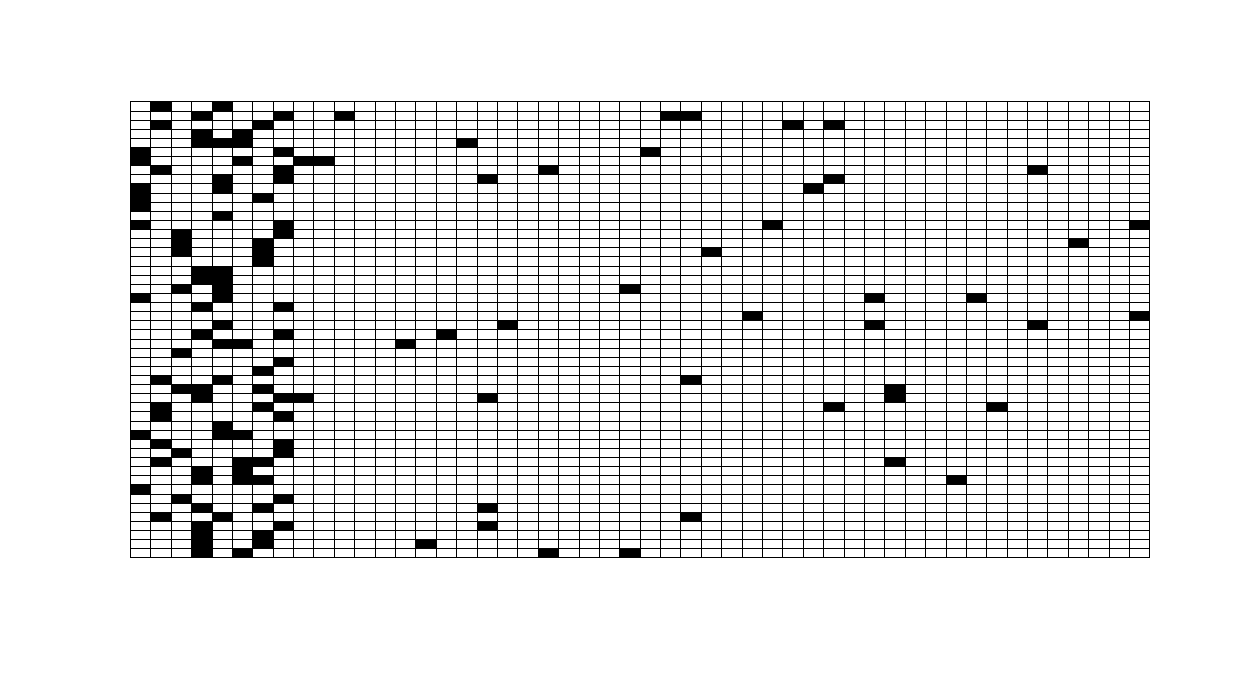
\includegraphics[width=0.8\linewidth]{eightdata.png}
\caption{Simulated Mutation Data}
\end{figure}
\end{frame}
\begin{frame}
Performance:\\
Set $t=2$, $k_{\min}=1$, $k_{\max}=6$, under the same device (My PC),\\
with relaxation of the problem, the linear programming was solved in about 1 minute, the result was not all integers.\\
First group:\\
0.5: 1,2,3,4,5,7,8,10,14,19.\\
1: 12.\\
0: others.\\
Second group:\\
0.5: 1,2,3,4,5,7,8,10,14,19.\\
1: 31.\\
0: others.\\
Without relaxation, time took: 0.05 second.\\
First group: 1,2,3,4,14,19.\\
Second group: 5,7,8,10,21,31.\\
\end{frame}
\begin{frame}
Performance:\\
Set $t=2$, $k_{\min}=3$, $k_{\max}=5$, under the same device (My PC),\\
with relaxation of the problem, the linear programming was solved in about 20 seconds, the result was not all integers.\\
First group:\\
0.5: 1,2,3,4,5,7,8,10,14,19.\\
0: others.\\
Second group:\\
0.5: 1,2,3,4,5,7,8,10,14,19.\\
0: others.\\
Without relaxation, time took: 0.02 second.\\
First group:\\
1,2,3,4,14.\\
Second group:\\
5,7,8,10,31.\\
\end{frame}
\begin{frame}
Set $k_{\min}=k_{\max}=4$.\\
Relaxation Problem: time 42 seconds.\\
First group:\\
0.5: 1,2,3,4,5,6,7,8.\\
0: others.\\
Second group:\\
0.5: 1,2,3,4,5,6,7,8.\\
0: others.\\
Without relaxation: 0.03 second.\\
1,2,3,4; 5,7,8,10.\\
\end{frame}

\end{document}
